\documentclass{standalone}
\usepackage{tikz}
\usetikzlibrary{calc}

\begin{document}

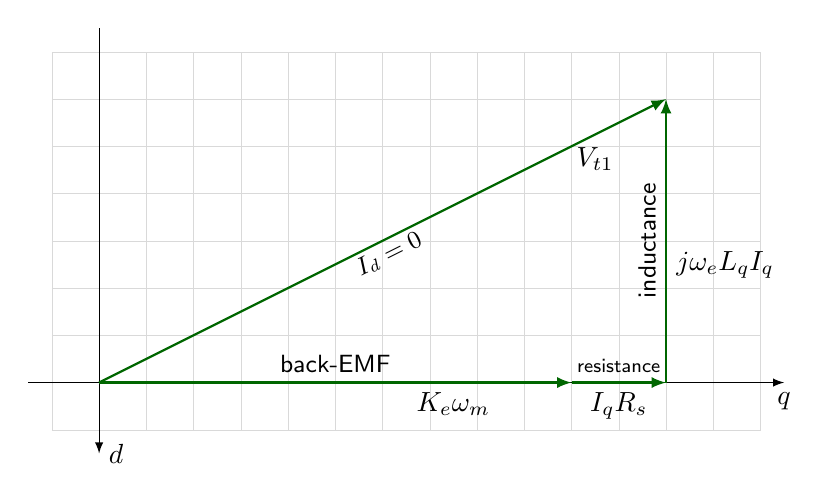
\begin{tikzpicture}[scale=3,>=latex]
\draw[step=.2cm,black!15,very thin] (-0.2,-0.2) grid (2.8,1.4);
\draw [->](-0.3,0) -- (2.9,0) node[at end, below] {$q$};
\draw [<-](0,-0.3) -- (0,1.5) node[at start, right] {$d$};

\definecolor{dkgreen}{rgb}{0,0.4,0}
\definecolor{dkblue}{rgb}{0,0.4,0.7}
\definecolor{dodgerblue}{RGB}{30,144,255}

\coordinate (V_bemf) at (2,0);
\coordinate (V_ir) at (0.4,0);
\coordinate (V_il) at (0,1.2);
\coordinate (V_bemfir) at ($(V_bemf)+(V_ir)$);
\coordinate (V_t1) at ($(V_bemfir)+(V_il)$);
\draw [draw=dkgreen, thick, ->] (0,0) -- (V_bemf) node[near end, below] {$K_e\omega_m$} node[midway, above] {\sffamily\small back-EMF};
\draw [draw=dkgreen, thick, ->] (V_bemf) -- +(V_ir) node[midway, below] {$I_qR_s$} node[midway, above] {\sffamily\scriptsize resistance};
\draw [draw=dkgreen, thick, ->] (V_bemfir) -- +(V_il) node[midway, below right] {$j\omega_eL_qI_q$} node[midway, sloped, above ]{\sffamily\small inductance};
\draw [draw=dkgreen, thick, ->] (0,0)--(V_t1) node[very near end, below=1pt]{$V_{t1}$} node[font=\small, midway, sloped, below=-2pt]{$I_d = 0$};
\end{tikzpicture}
\end{document}